% !TEX encoding = UTF-8 Unicode

\documentclass[twocolumn,10pt,a4j]{ltjsarticle}
\usepackage{kougai}

\title{初学者向けネットワーク通信の学習を支援するWeb教材}
\author{1932047 小松崎 嵩史  指導教員 須田 宇宙 准教授}
\date{}

\begin{document}

\maketitle

%1章
\section{はじめに}

%背景
DX(Digital Transformation)の実現に向けて,IT人材の確保・育成は大きな課題となっている\cite{dx}.
IT人材の確保・育成のため,2020年より小学校から始まる情報教育の推進が図られている.
高等学校においても新しい学習指導要領が改訂され,「情報Ⅰ」が共通必履修科目となっている.

%問題点

情報教育の学習内容において,ネットワークの学習はプログラミングに比べて,講義形式の授業が多くなる点が問題点として挙げられる.
実習形式での授業が難しい理由として,学習指導要領でプログラミングを実習形式で学ぶことが勧められていること,ネットワークの実習に,通信機器,仮想環境などの準備が難しいことが考えられる.
講義形式の授業では,初学者がネットワーク通信の層の動きや違いを,紙面の文字や図だけで理解することは難しいと考えられる.

%目的
この問題に対して,生徒や学生に配布されるタブレットや,小型のPCで利用できるWeb教材を講義形式の授業の補助に利用することで,問題点の改善に繋がると考えた.
本研究では,上記のWeb教材を作成することを目的とする.

%2章
\section{本研究に関連する教材について}
本研究の目的と類似するものとして,電子版の教科書や教科書のQRコードを読み取り利用する,教科書付属のアニメーション教材が存在する.
この教材の問題点として,短いアニメーションと文字のみで解説文との対応が無いこと,高等学校において電子版の教科書が普及していないことが挙げられる.

%3章
\section{本教材の学習内容について}
高校の科目「情報Ⅰ」の学習内容「ネットワークのプロトコル」から,「カプセル化」,「パケットの構造」,「下位層の役割」を学習する.
本研究で開発したWeb教材は,ネットワークの基礎であるTCP/IPとOSI参照モデル,データリンク層とネットワーク層を学習する授業で利用されることを想定している.

%4章
\section{開発した教材について}
利用環境は,生徒や学生に配布されるタブレットや,小型のPCを想定している.小さな画面における視認性や操作性を考慮して画面を設計した.
メインとなる図や解説文は,拡大縮小やスクロール操作を行わずに操作できるようにしている.
また,ネットワークの学習において用語が多く登場するため,図や解説文を崩さずに用語解説を見ることができるようにしている.
そして,小さな画面で大量のボタンや操作部分を配置すると複雑になりすぎるため,解説中心の「学習画面」,学習者が値を設定して動かす「シミュレータ画面」で分けてページを構成している.

作成したWeb教材の「学習画面」の例を図\ref{fig:画面}に示す.
①は,「学習画面」か「シミュレータ画面」を選択するナビゲーション部である.
②は,図やアニメーションが表示されるメイン表示部である.
③は,②の操作に対応した解説文を表示する解説表示部である.
④は,③内の用語を解説する用語解説部である.

作成したWeb教材の「シミュレータ画面」の例を図\ref{fig:画面2}に示す.
⑤は,シミュレータのアドレスや通信方式の設定を行うシミュレータ設定部である.

\begin{figure}[h]
\begin{center}
 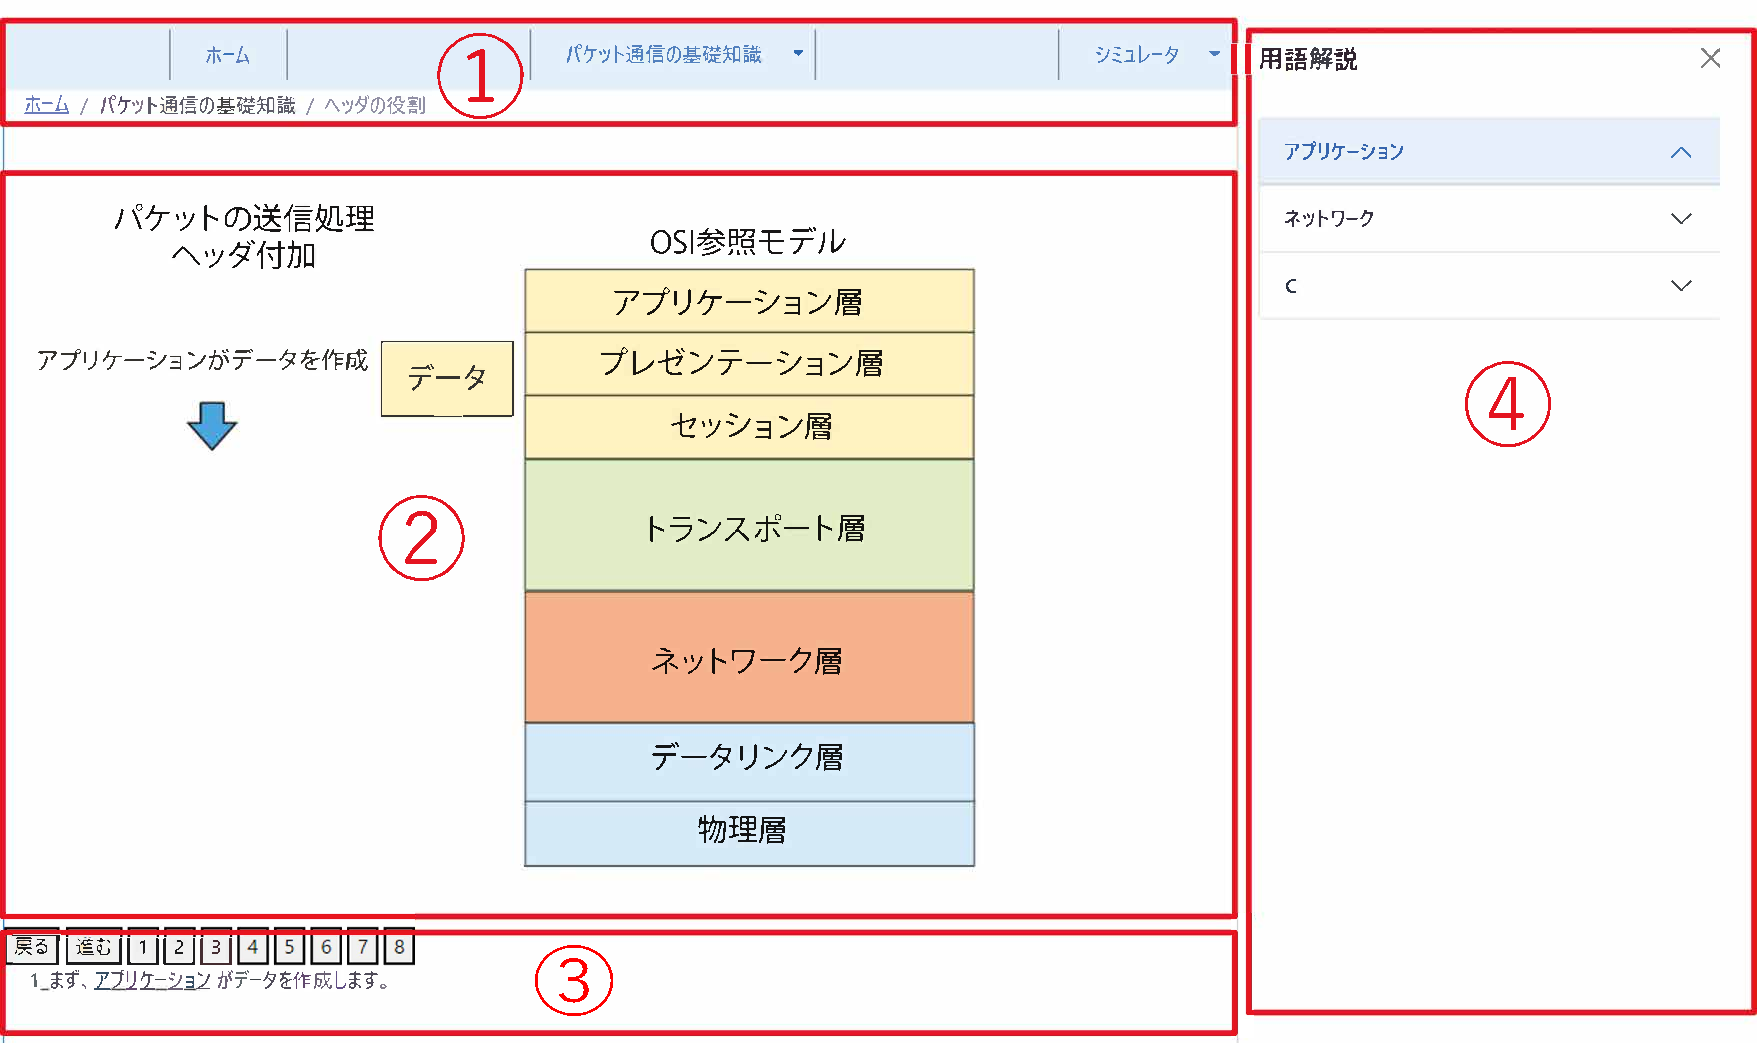
\includegraphics[clip,width=82mm]{figures/gamen.pdf}
\end{center}
 \caption{Web教材の学習画面}
 \label{fig:画面}
\end{figure}

\begin{figure}[h]
\begin{center}
 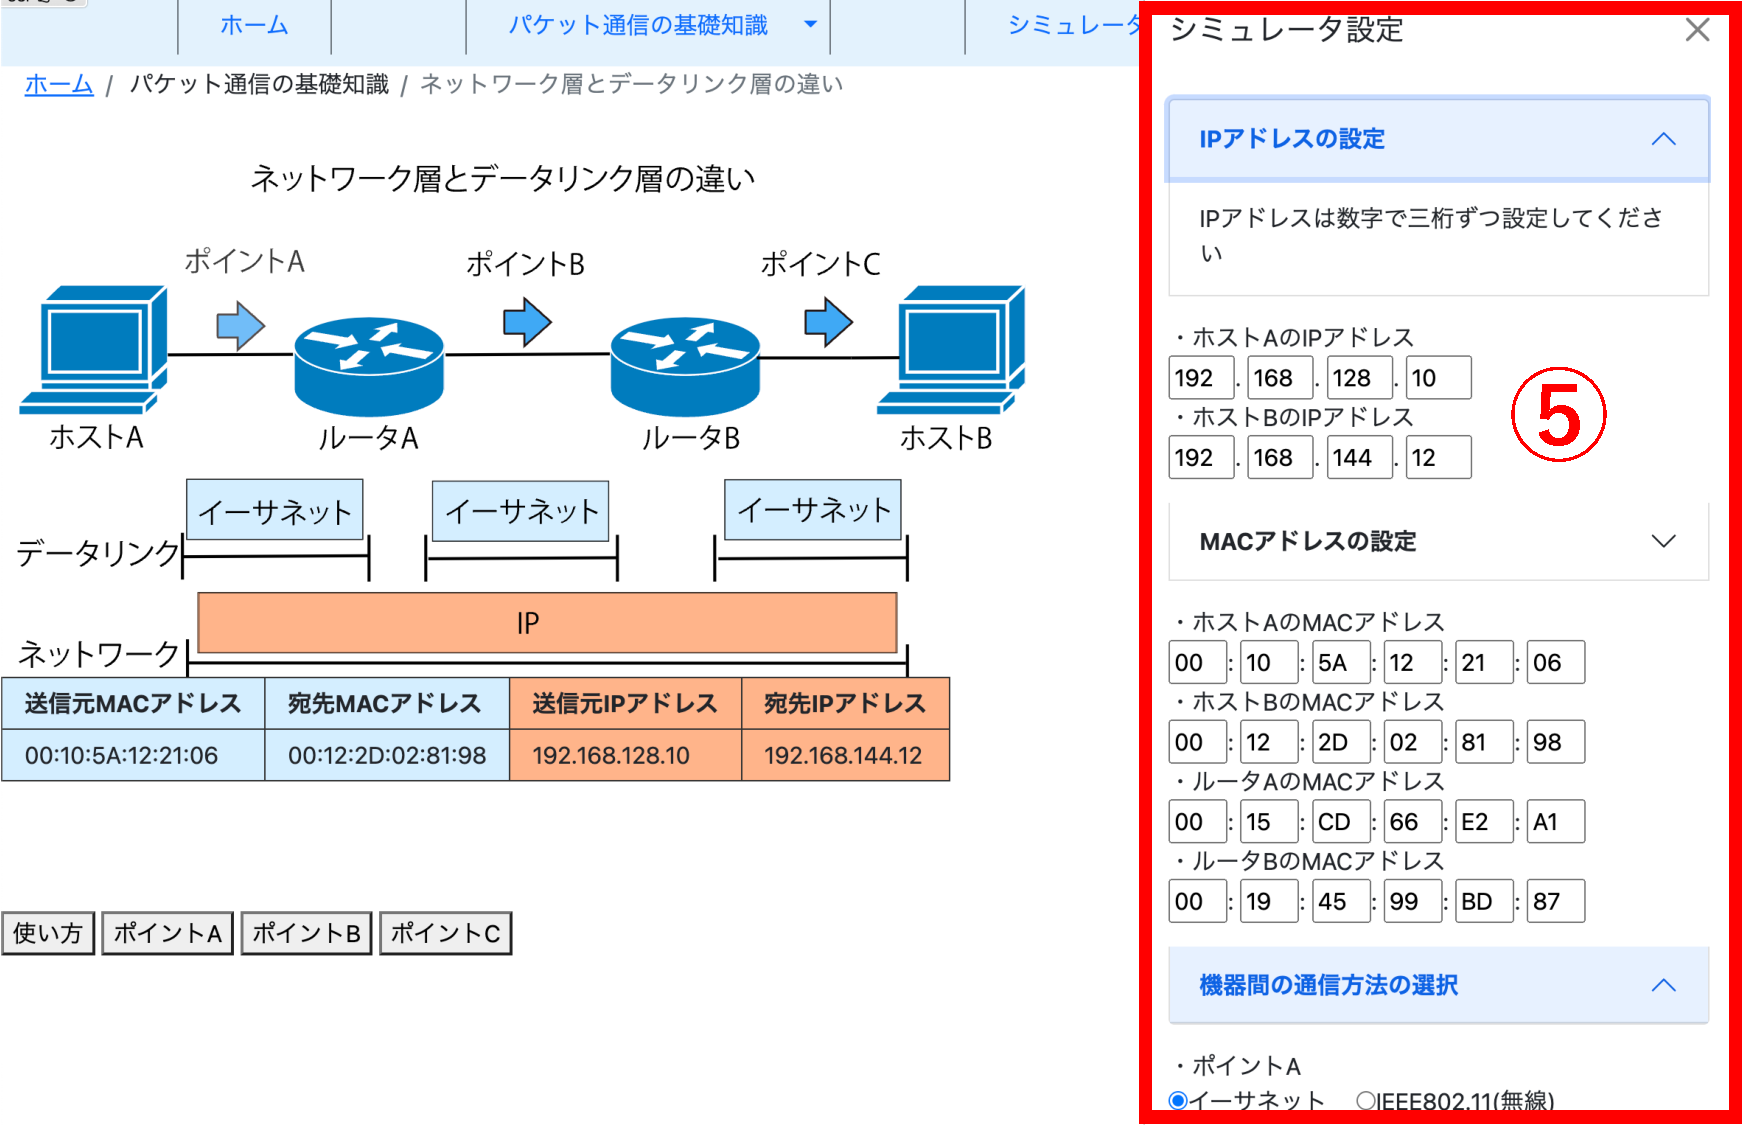
\includegraphics[clip,width=82mm]{figures/gamen2.pdf}
\end{center}
 \caption{Web教材のシミュレータ画面}
 \label{fig:画面2}
\end{figure}

%5章
\section{おわりに}
本研究では,ネットワーク通信の基礎を学習する講義形式の授業を補助するWeb教材を開発した.今後このような,生徒や学生が自ら操作し学習できるWeb教材が普及し,ネットワーク通信の基礎を容易に理解できるようになることを期待している.

\begin{thebibliography}{99}
\bibitem{dx} 総務省: ``令和4年度版 情報通信白書'', p101, \url{https://www.soumu.go.jp/johotsusintokei/whitepaper/ja/r04/pdf/n3800000.pdf}, 2022/12/12参照

\end{thebibliography}

\end{document}
